\documentclass[border=6pt]{standalone}
\usepackage{fontspec}
\setmainfont{TeX Gyre Termes}
\usepackage{tikz}
\usetikzlibrary{arrows.meta,positioning,fit,backgrounds}
\definecolor{navy}{HTML}{16324F}
\definecolor{blue}{HTML}{2F6690}
\definecolor{green}{HTML}{3A7D44}
\definecolor{orange}{HTML}{D17A22}
\definecolor{red}{HTML}{A23E48}
\definecolor{lightblue}{HTML}{EAF3F8}
\definecolor{lightgreen}{HTML}{EAF5EC}
\definecolor{lightorange}{HTML}{FFF2DF}
\definecolor{lightred}{HTML}{FBEAEC}
\tikzset{
  box/.style={draw=navy, very thick, rounded corners=2pt, align=center, font=\small, inner sep=5pt, minimum height=0.9cm},
  data/.style={box, fill=lightblue, text width=2.25cm},
  calc/.style={box, fill=lightgreen, text width=2.25cm},
  agent/.style={box, fill=lightorange, text width=2.5cm},
  control/.style={box, fill=lightred, text width=2.5cm},
  arrow/.style={-{Latex[length=2.5mm]}, very thick, draw=navy},
  danger/.style={-{Latex[length=2.5mm]}, very thick, draw=red, dashed},
  label/.style={font=\scriptsize, align=center, fill=white, inner sep=2pt},
  participant/.style={box, fill=lightblue, text width=2.3cm, minimum height=0.75cm},
  zone/.style={box, minimum height=1.1cm, text width=4.1cm},
  smallbox/.style={box, font=\scriptsize, text width=3.5cm, minimum height=0.7cm}
}

\begin{document}
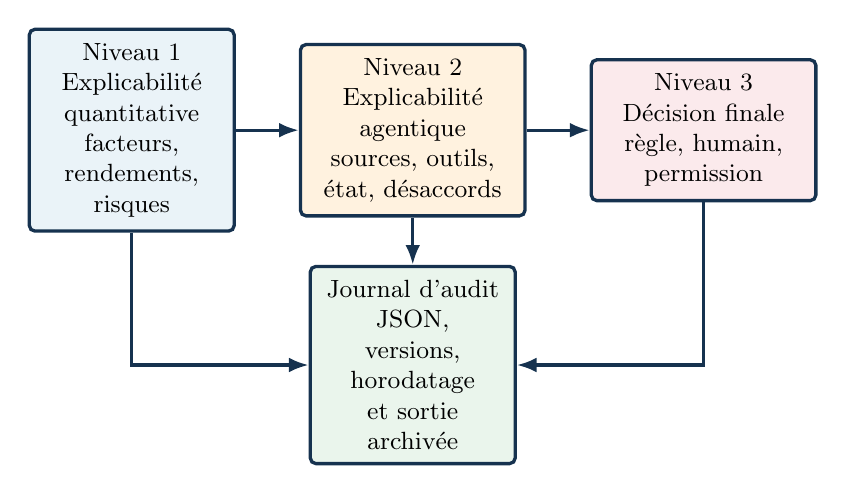
\begin{tikzpicture}[node distance=6mm and 8mm]
\node[data] (q) {Niveau 1\\Explicabilité quantitative\\facteurs, rendements, risques};
\node[agent, right=of q] (a) {Niveau 2\\Explicabilité agentique\\sources, outils, état, désaccords};
\node[control, right=of a] (d) {Niveau 3\\Décision finale\\règle, humain, permission};
\node[calc, below=of a] (audit) {Journal d'audit\\JSON, versions, horodatage\\et sortie archivée};
\draw[arrow] (q) -- (a);
\draw[arrow] (a) -- (d);
\draw[arrow] (q.south) |- (audit.west);
\draw[arrow] (a.south) -- (audit);
\draw[arrow] (d.south) |- (audit.east);
\end{tikzpicture}
\end{document}
